\chapter{Experiences of Science Capital in University Science}

\section{Preamble}
The following chapter details the results of a set of nineteen interviews that were conducted with science students at the university of Auckland. I mirror the structure of the previous chapter, where I outline arguments for a conceptual model of how capital is accumulated by students as university. The current chapter, in addition to detailing the qualitative methodologies employed, will seek to add the colour of life experiences to my conceptual model. It is in this chapter where I seek more understanding of \textit{why} students do choose to study science. In order to answer the question of why, I seek to answer three more specific research questions:
\begin{itemize}
    \item What forms of social capital are available to university science students? 
    \item How do students leverage social capital to gain advantage in the field of university science? 
    \item How does students' habitus contribute to the accumulation of capital?
\end{itemize}


\section{Methods}
I adopted a staggered research design, with the research process taking place over three separate phases. As shown in Table \ref{tab:Phases}, the process began with four interviews with students in the science scholars programme (a programme for gifted science students) at the UoA. Based on preliminary data from these interviews and a questionnaire provided by the ASPIRES research group in the United Kingdom \citep{dewitt2011high}, a questionnaire was designed to assess the relationships between students' social capital, cultural capital, social location (gender, ethnicity, socio-economic status), and confidence in science. The questionnaire asked students to record factual information about themselves, and answer items regarding 5 latent constructs informed and adapted from the work of \cite{dewitt2011high}. The constructs included self-concept in science (Science Self-concept), experience of high school science teachers (Science Teachers), parental attitudes towards science (Science Parents), peer attitudes towards science (Science Peers), and access to science-related resources (Science Resources). Results of a Confirmatory Factor Analysis (CFA) provided support for these 5 factors ($\chi^{2} =$ 483.74, $\mathrm{df} =$ 179, p $<$ .001, CFI  $=$ 0.93, TLI  $=$ 0.91, RMSEA $=$ 0.05), while separate tests of showed adequate reliability of each construct (McDonald's $\omega$ 0.68 - 0.86). More detailed information regarding questionnaire design and quantitative results is available in Chapter 4. 
\begin{table}[ht]
\begin{tabular}{c|c|l}
                      
Phase  & Year & Purpose    \\ \hline
1   & 2018  & Interviews with 4 high achieving science students at UoA.     \\
& & Results of these interviews were used to inform questionnaire design. \\ \hline
2  & 2018-2019 & Questionnaire design and administration to science students at UoA.  \\
& & Questionnaire analysis conducted (see Chapter 4)\\ \hline
3 & 2019 & Main interviews conducted with 15 students. \\
& & These were selectively sampled from the questionnaire. \\ \hline
\end{tabular}
\caption{\label{tab:Phases} The timeline of the qualitative research process. Preliminary interviews with four high achieving science students informed the design of questionnaire, which was administered to science students at UoA in early 2019. Fifteen students were then purposefully sampled for interviews based on questionnaire responses.}
\end{table}

The staggered research design has been used in previous research to investigate student experiences in STEM to great effect \citep{grossman2014perceived,russell2011factors}. Whereas previous research has focused on random sampling \cite{russell2011factors} or purposeful sampling to achieve a balance of gender or ethnicity in interviews \citep{grossman2014perceived}, the current study seeks to take a more intersectional methodological approach by including domain-specific indicators of social class as well as self-report measures of gender and ethnicity in the decision making process. The following section will outline the methods used in the interview phases in more detail.

\section{Methods}
The current study draws from the pool of questionnaire respondents . As shown in \ref{fig:ScienceFactors_C6}, students were purposefully sampled from a range of different social locations, with the aim of representing a range of student experiences. 

\begin{figure}[ht]
\centering
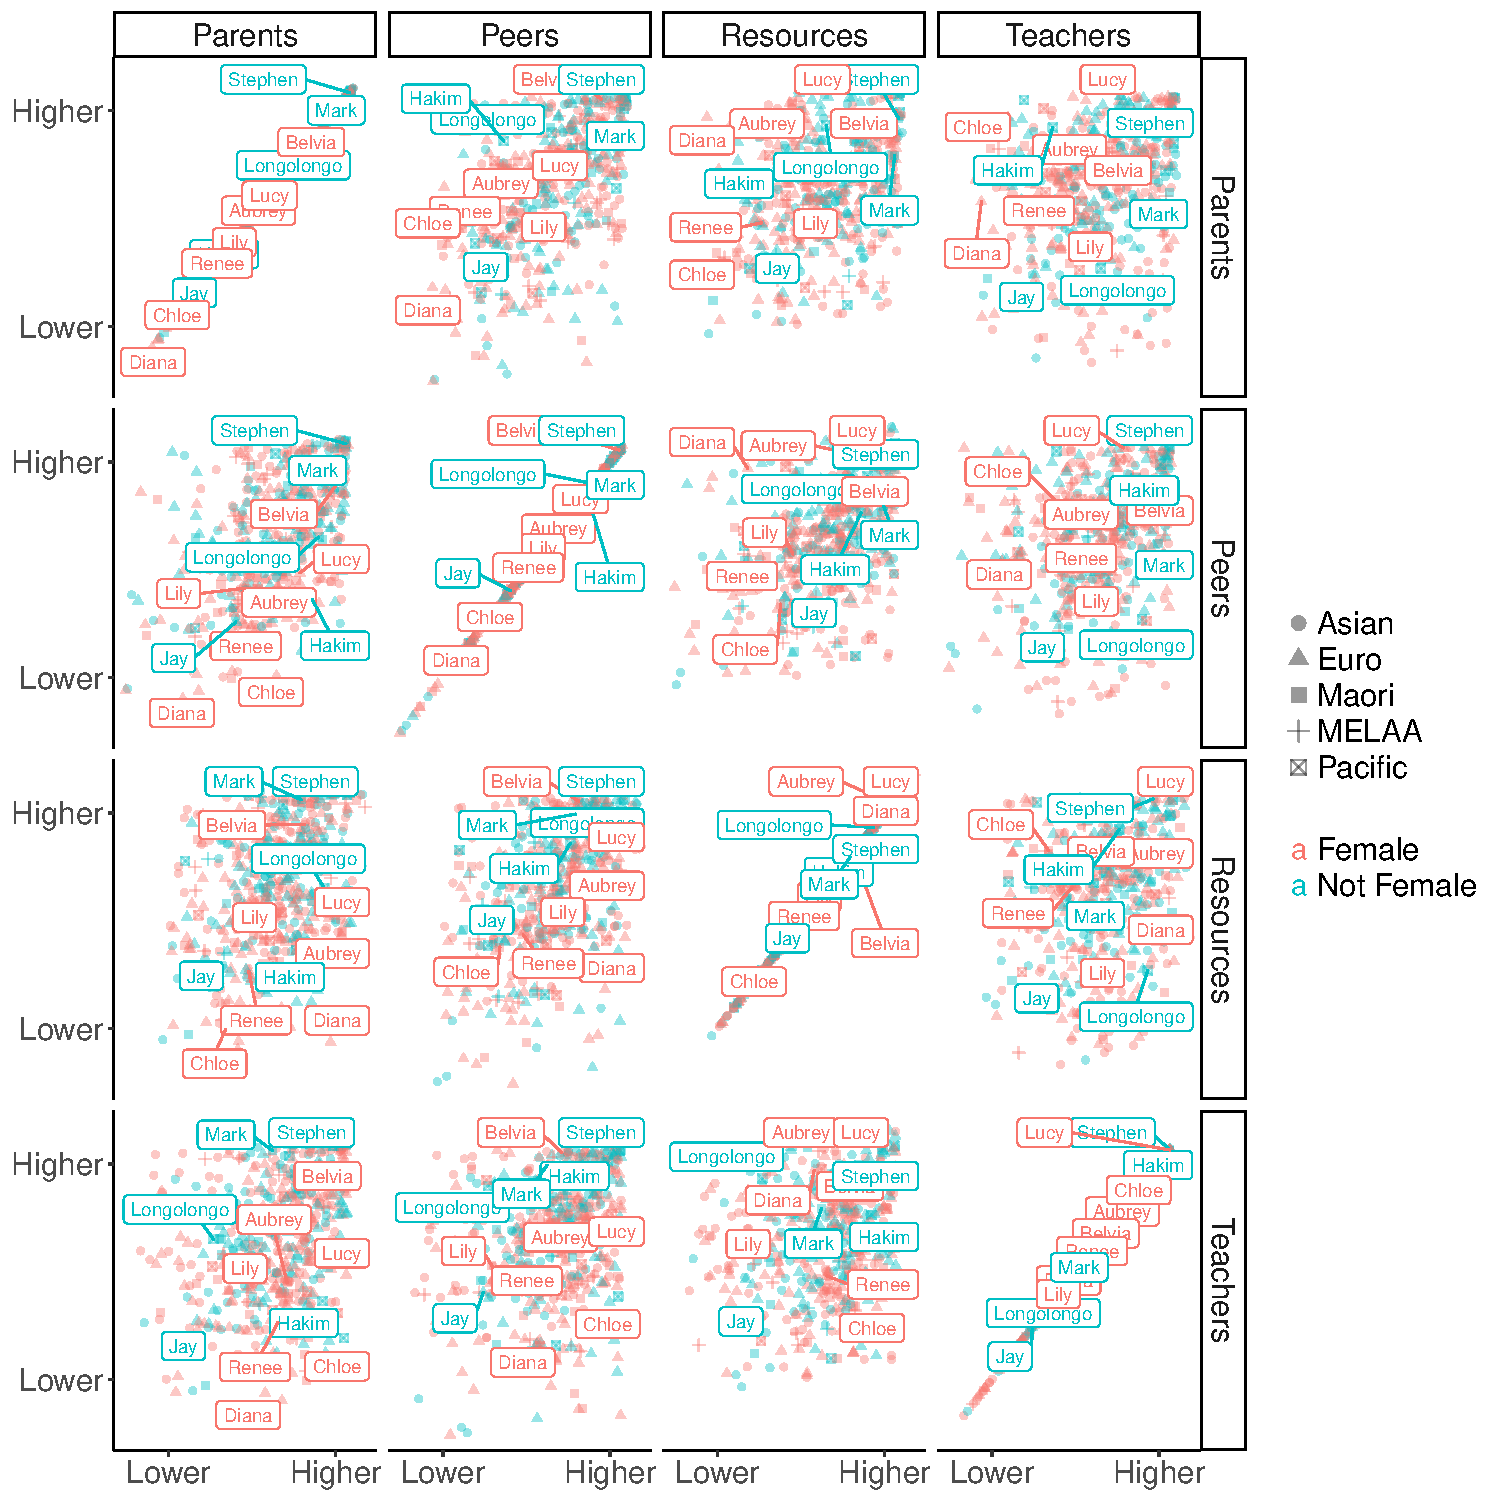
\includegraphics[width=\textwidth]{C6 - Experiences of Science Capital/ScienceFactors_FacetPlot.pdf}
\caption{\label{fig:ScienceFactors_C6}\textbf{Sampling Strategy}. The above plot shows the methods used to sample students when arranging interviews. I aimed to interview students with a range of different backgrounds with regards to forms of science capital. Axes indicate the students' level of a particular form of capital, including Science Parents, Science Peers, Science Resources, and Science Teachers. The locations of 12 of the 19 interviewee participants are highlighted by their pseudonym. The four participants interviewed at phase 1 are not included, while three interview participants from phase 3 were excluded from factor analysis due to having too much missing data in the questionnaire (see Chapter 4). Individual data points are also coloured and shaped at the intersection of identified gender and ethnicity. In this case, ethnicity is coded according to prioritised ethnicity, where students who identified with multiple ethnicities were first coded as M\={a}ori, then Pasifika, then Asian, then European (following guidelines set out by Statistics New Zealand). I only use the prioritised ethnicity for ease of plotting and not for any analysis. Gender in this case refers to whether the individual self-identified as female or not. }
\end{figure}

Given the goal of these interviews is to reveal variation in the students experiences in science, rather than to discuss the properties of a `sample', it can be argued that a sample size of 19 participants is sufficient \cite{berglund2006students}. For participants drawn from the questionnaire, sampling was prioritised based on the constructs of capital measured in the questionnaire (Figure \ref{fig:ScienceFactors}), and also according to whether they identified as a member of an underrepresented social group in science. The purposeful sampling was a deliberate choice informed by research on intersectionality. As outlined by \cite{duran2019using}: ``Even if multiple marginalized demographics are not the subject, they must always be centered.'' The social groups I intentionally sampled were thus as follows:
\begin{itemize}
    \item Individuals with lower levels of science related capital. This judgement was made based on students reported scores on the teachers and peers value of science constructs, which were found to be the most important predictors of self-concept in science in Chapter 4.  I also took into account other indicators of science-related capital, such number of books at home growing up and access to science related activities.
    \item Individuals with parents who do not value science, or who do not talk about science often. Even though parents value of science was not a significant predictor of science self-concept in Chapter 4, I expected it to still play a major role in participants' development of habitus in science. 
    \item First generation to university students. 
    \item M\={a}ori and Pasifika students. While research has explored factors relating to success at university in general for students identifying as M\={a}ori and/or Pasifika \citep{mayeda2014you}, there is a need for research that seeks to present their experiences in science specifically. 
    \item Female students in physics and computer science. Through interviews with these students we may begin to describe why we see certain trends in student enrolments, such as those described in Chapters 2 and 3.
\end{itemize}
While the above criteria represent the students of specific interest, the students interviewed represented a range of social backgrounds, with some students representing multiple criteria and some not representing any. It is also important to note that the categories employed are simplistic and do not encompass a range of other important characteristics (such as religion or ableness), or indeed the complexity of belonging to multiple groups. While much research of marginalised groups in science is grounded in deficit-theorising (why do students drop out?), the current study attempts to adopt an asset-based framework (why do students succeed?). This framing is prefaced by the acknowledgment that while resilience should be celebrated, it should not be necessary. Participant characteristics are summarised as in Table \ref{tab:Demographics} and participant summaries are also available as supporting information. 


\begin{table}[ht]
\begin{tabular}{cc|c}
                       &                        & Count \\ \hline
Gender                 & Male                   & 7     \\
                       & Female                 & 8     \\ \hline
Ethnicity              & Asian                  & 3     \\
                       & M\={a}ori                  & 7     \\
                       & Pasifika               & 3     \\
                       & Pakeha/European        & 9     \\ \hline
University Generations & First Generation       & 7     \\
                       & Sibling                & 2     \\
                       & Parent                 & 4     \\
                       & Grandparent and Parent & 2     \\ \hline
Subject Disciplines    & Biology                & 8     \\
                       & Chemistry              & 7     \\
                       & Computer Science       & 6     \\
                       & Mathematics            & 3     \\
                       & Physics                & 7     \\
                       & Psychology             & 3     \\
                       & Statistics             & 4     \\ \hline
Self-concept          & Higher                   & 7     \\
                       & Lower                    & 5     \\ \hline
Science Parents        & Higher                   & 8     \\
                       & Lower                    & 4     \\ \hline
Science Teachers       & Higher                   & 7     \\
                       & Lower                    & 5     \\ \hline
Science Peers          & Higher                   & 7     \\
                       & Lower                    & 5     \\ \hline
Science Resources      & Higher                   & 8     \\
                       & Lower                    & 4    
\end{tabular}
\caption{\label{tab:Demographics} A table summarising the characteristics of the individuals who participated in interviews following completion of the questionnaire. Aggregated group counts are provided to help preserve anonymity. Participants may have identified with multiple ethnicities or be enrolled in multiple subject disciplines, which means that these counts do not sum to fifteen. Three students who participated in interviews did not provide enough information on construct items to have scores on self-concept and capital scales attributed to them. Information is not presented for the four students who completed the first interview phase of the study, prior to administration of the questionnaire.}
\end{table}

\subsection{Qualitative approach and research paradigm}
Interview questions were based on the items presented to participants in the questionnaire. These questions reflect a deductive approach, where previously established theory guides questions. This process was conducted explicitly by using the participants' questionnaire responses as an object for discussion. For example: 
\blockquote{On this section: my friends see me as a science person. You scored quite highly - how do you feel about that?} While interviews were directed by participants' questionnaire responses, they were also semi-structured. This means that participants were encouraged to lead discussion and talk about what they felt was important. As M\={a}ori were invited to be interviewed, this inductive approach was informed by Kaupapa-M\={a}ori-Consistent (KMC) practices. KMC practice requires research concerning M\={a}ori to be conducted with, and not on, M\={a}ori \citep{walker2006exploration}. My attempts to adhere to KMC practices meant that the conceptualisation and operationalisation of research procedures were also discussed with M\={a}ori representatives. Echoing the procedures of \citet{mayeda2014you}, questions regarding sensitive topics, such as personal experiences of discrimination, were avoided. While many participants did discuss these types of experience, they had power and agency to share those experiences. Participants were also offered transcripts of interviews and manuscript drafts, and invited to remove, edit, and add responses after the interview.  

An inductive approach to thematic analysis was used to analyse the interview transcripts, following the general guidelines set out by \cite{Braun_2006}. Interviews were coded in accordance to the the three established research questions:  what forms of social capital are available to university students? How do students leverage social capital to gain advantage in the field of university science? And finally, how does students' habitus contribute to the accumulation of capital? Themes were then established and developed into the conceptual model outlined in Chapter 5 to aid in answering these questions. Bourdieu's sociological theory was employed as a conceptual ``toolbox'', drawing primarily on his concepts of social capital, habitus, field and doxa. The conceptual model (Figure \ref{fig:HabitusSocCap_TheoreticalModel_C6}) provides a lens to explore how social capital impacts on habitus, and how habitus then influences future capital accumulation. 

\begin{figure}[ht]
\centering
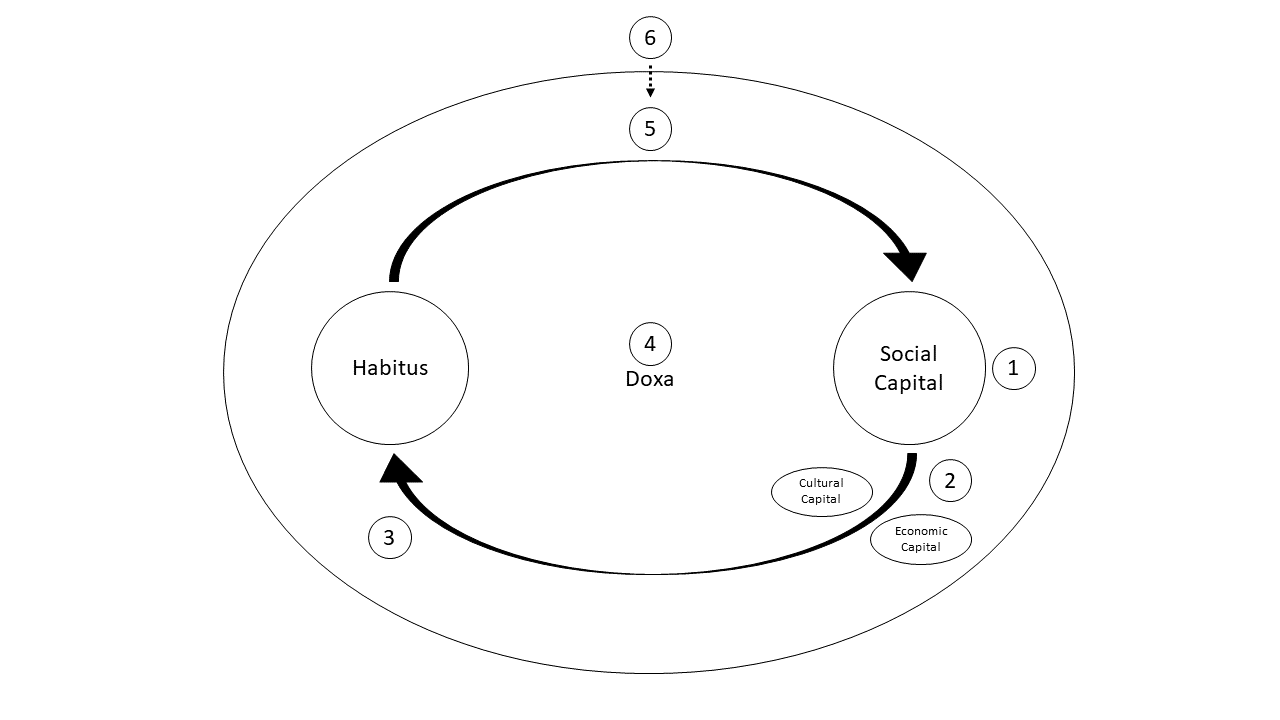
\includegraphics[width=\textwidth]{C5 - Understanding Capital Accumulation/HabitusSocCap_TheoreticalModel.png}
\caption{\label{fig:HabitusSocCap_TheoreticalModel_C6}\textbf{Conceptual Model}. The conceptual model used to understand individual practices in the field of science education. The model, informed by the experiences of participants in the current study, expands on the interaction between habitus and capital originally illustrated by \cite{Bourdieu1984}. The model provides a step by step description of how social capital translates into habitus transformation, and how habitus generates future capital accumulation. Step 1 refers to the initial availability of social capital for an individual. Step 2 refers to the value gained through leveraging social capital into forms of economic and cultural capital. Step 3 refers to how social capital is internalised by the individual. Step 4 refers to how habitus informs the acquisition of future social capital. 5 refers to factors outside of the individual that structure the field (by availability of capital and exchange value).}
\end{figure}

The following sections will describe the perceptions of participants, following the structure of the conceptual model outlined in Chapter 4. While much of my discussion simply describes the experiences that participants reported (semantic themes), the goal of my analysis is to be interpretative \citep{Braun_2006}. This means that I intend to go beneath the level of description and to place participants' experiences into the conceptual model, which I theorize shapes the experiences of participants. Prior research is referenced to support my interpretations. 

\section{Social Capital in the Field of University Science (Step 1)}
This section discusses the availability of social relationships that participants had in the field of university science (Step 1 in Figure \ref{fig:HabitusSocCap_TheoreticalModel_C6}). These relationships are categorised into three key groups, social capital through family connections, social capital through educators, and social capital through peers. 

\subsection{Family, Whanau, and Significant Others}
Students' upbringing within the their family and whanau was an important influence on their experiences of university science. The M\={a}ori term \textit{whanau} refers to extended family or a community of related families, and therefore this theme refers to the social capital student's held via their parents and siblings, but also through aunties, uncles, and grandparents. Access to social capital through family differed across participants. Some participants came from highly academic families with science backgrounds, others had whanau with little experience of science education. 

Some participants had family that were interested in science and were available to  talk about it. Participants, like Susan, remember hearing their parents talking about science from an early age: ``my parents loved to talk about it. I was very excited when I learned you could do maths at university when I was about 10.''  Even if parents do not explicitly endeavour to talk to their children about science, having an academic background may enable them to do so. Sean, who's mother worked in a science lab, recalled: \blockquote{I haven't really had much science discussions with my parents, but when the science questions do come up between me and my sister then they sort of hop in.} Many participants felt their parents held an interest in science, even if they did not study it at school. Patrick recalled the interactions he would have with his father growing up: \blockquote{My dad used to watch science documentaries all the time just because he found it interesting or whatever. I used to talk to him about stuff like that.} With that being said, Patrick felt that he did have fewer opportunities to talk about his university degree and plans for the future: \blockquote{most of the time he doesn't know what I’m talking about, but he will still listen to what I’m talking about...  I just have no one to [talk to] really.}

In other cases, participants felt that their family did not hold interests in science. It may be that while a general form of social capital within the family is available, social capital that is valued in the field of university science is not. Chloe recalled that her family, who valued education and other academic fields, did not see value in science: \blockquote{my family isn't interested in science and that is cool, I am not interested in banking... I think they have no idea of science because they don't do science, so they don't really know what science is so it is kind of like not normal to my family}. Many participants felt that their family was indifferent to science, such as Aubrey. She felt that her parents ``switched off'' whenever she tried to talk to them about science: \blockquote{I try to tell them something and they go oh that is nice and just kind of start talking about something else.} 

In other cases, family may have a direct negative impact on participants' learning. Some participants found they needed to step away from family, whanau, or significant others who did not value science education in order to aid their educational journey. Renee identified the moment that she left a controlling partner as a key moment in their pursuit of education: \blockquote{It is like when you hold a spring down and it has got so much potential and then you let it go and it is like fuck yeah, do you know what I mean? Like that was me leaving that person and being like `yeah'.} Leaving a relationship where values regarding education are not shared gave Renee a renewed sense of potential. Hakeem, who's comes from a strongly family-orientated Pasifika family, found that moving into his own space allowed him to focus more on his education:
 \blockquote{I got my own place which is huge. I’m living out west now away from my parents, just having that kind of space and gap from your family it was really huge for me. Yeah just the quiet time and the solitary. I needed that space from everyone because I had been around family, really family orientated family and they are really close connected. They want to hang out all the time they want to do this. Yeah I just liked having my own space... It was a good environment for studying in. Results have improved a bit since the start of my computer science journey.
 }
Hakeem's experience has been similarly echoed in prior research which suggests that family responsibilities place more demands on Pasifika and M\={a}ori students \citep{zepke2011non}. In a study of post graduate Pasifika university students, \cite{theodore2018pacific} found that family responsibilities were the most commonly cited factor that hindered qualification completion. With that being said, the support of family was the most cited source of help for students, a finding that is also reflected in the experiences of participants in the current study (to be discussed in section 6.5.1). 


\subsection{Educators}
The relationships participants shared with their high school teachers, university tutors and lecturers were highly influential in shaping students experiences of university study. Some participants had teachers who were good sources of social capital as they had expertise and knowledge on what was needed to progress to university science. The perceived availability of educators varied for each of the participants, with this being informed by participants' knowledge of how to approach them, and participants' perception of how approachable the educators were. 

The availability of social capital through educators can be driven by students and/or driven by educators. Sean identified that it was his responsibility to approach his teachers when he needed help: \blockquote{All our teachers were way good, so you always had really good teachers and it was just up to you to get what you wanted, just get what you wanted out of them.} With that being said, participants found it easier to make connections with educators when they felt they were approachable. Alicia, remembered how, even when she did poorly in English, her teacher helped her stay motivated: ``the teacher always encouraged me that you can do well, and I liked her personality and beyond of just studying subject I have more personal attachment to that person.'' The importance of personal attachment was echoed by Stephen: \blockquote{I think the fact that we all could engage in a conversation with him is probably the best thing that a teacher could have}. Belvia found that having lecturer who is friendly and patient made ``a big difference'' to her learning: \blockquote{if someone asked a question in class he would be like `oh yeah this is how you do it'. He would like draw it out and take his time to actually explain}. Belvia was unable to leverage the same value from a social relationship with another lecturer who did not want to answer her questions straight away: \blockquote{he would just go straight onto --- okay I'll see him later and ask him. I don't know, but how can you ask him, you are going to forget... I don't know man. It just felt like he did not care.} Belvia's experience demonstrates how perceptions educators' availability is informed by an educator's actions. The more a students perceives a positive relationship with their educator, the more social capital they have available. 

Participants appreciated having teachers who would check in with them and make sure they were on track. Jay recalled how his calculus teacher would ``consistently walk around the class ask if you need help''. Jay's example demonstrates how educators can make themselves explicitly available to their students. Educators may make themselves more available to students at high school, while this might be less common at university where independent learning is more expected. Lily discussed the transition to more independent learning at university: \blockquote{Obviously you are in lectures, it is not just a classroom and it is very independent learning, and lecturers are not always on your back saying `you need to get this in' or `this is overdue, why is it overdue'.
} Lily's experience describes how the availability of social capital with educators may lessen with the change in field. After transitioning to university study, students may be more unsure about how to approach their educators. Some participants were aware that the rules may be different to high school, and that there may be different conventions to follow when communicating with lecturers or tutors. Paul, a science scholar with mentors at university, did find it difficult to know what conventions to follow:
\blockquote{I haven't emailed anyone. I think about it, but again I don't know how I am supposed to approach anyone... I'm never really sure how things work in a university environment, how polite can you be, how do you contact these people in the first place}. Accessibility is thus influenced by the students perception of their educator, the educator's own volition, and also the conventions of the field. Students who are most aware of the conventions to follow will be the most able to acquire social capital. 

The availability of educators may also relate to classroom structures that make it difficult for students to connect. Patrick found that he was not taught much in one of his university classes where lots of students were present: \blockquote{We had a class, a lecture, and most of the lectures were just big tutorials. We weren't taught anything. The teacher would just walk around in a class of about like 80 and we just didn't really learn anything. So we kind of got a bad impression from that class.} 

Educators may also be perceived as intimidating and unapproachable regardless of the classroom structure. These feelings of intimidation may be based on explicit past interactions, as described by Belvia: ``[the lecturer] definitely did not care because he was like so ruthless. He was like no that is a dumb question.'' Similarly, Patrick signalled that lecturers may have developed a poor reputation which makes them unapproachable to many students: \blockquote{he used to like not really be rude but give really blunt answers. Yeah so students didn't really ask him much and he kind of has a reputation for being kind of a hard guy.} 

\subsection{Peers}
Participants recalled varied experiences of the networks of peer relationships open to them. Unlike educators, from which the value of social capital is mainly derived in an academic context, the value of social capital from peers can be both academic and non-academic. While some participants entered into university study with a cohort of students from the same school, other participants entered university with limited peer networks. This tended to be the case for participants who attended high schools located in different geographic regions to the UoA, or for participants from high schools where university was not a common or expected pathway. 

Participants who originated from geographic regions outside of Auckland may enter into UoA with fewer connections. Stephen found the move from a rural area to Auckland difficult: \blockquote{It was harder this time to transition back into the city life though, because going from the small town only four or five people from my school came to Auckland.} Of these students, Stephen was the only one studying science, which put more pressure on him to make friends with people he did not know: \blockquote{I didn't know anyone doing science especially my major. No one I knew from my old schools... I was kind of pushed into that idea of having to make new friends and having to try and socialise with people that I didn't know.} The feeling of being ``pushed'' signals the discomfort that some students may feel when placed in a situation outside of their comfort zone, and highlights the added stress that may be experienced for students entering into university without an existing peer network of support. In contrast, some participants entered into university with a cohort of their friends from high school. Belvia entered into university with many friends, many of which have since graduated: \blockquote{since most of my friends have gone I have only like four of my original friends here, and shit everyone is graduating I need to get out of here. I need to actually start moving on with my life and stop being in the comfort zone of mine.} Belvia's trepidation with regards to her declining peer network at university points to the important role that peers play. 

The structure of physical spaces at high school and university may facilitate or hinder students' access to social capital through their peers. Some participants who stayed in student flats or university accommodation were connected with other students based on physical proximity. Mark suggested that staying in the same space made it easier to make connections with others studying the same degree: \blockquote{Since I’m staying at halls there are lots of engineers within my own floor. So we are able to just casually if we are in the common room can all get together}. Tutorials may also also give students the opportunity to make connections with other students. Belvia recognised it was easier to make friends in tutorials as opposed to lectures: \blockquote{I would try and make friends mostly in the tutorials because that is a smaller group. I feel like it was too hard to make friends in lectures because you would sit next to a person in the first few weeks and I’m shy and you don’t see them again. It is not like you are going to be talking to them after the lecture like let’s hang out now.} Belvia's experience points to the need for time as well as proximity as a key factor in the development of social relationships. A lecture, often a highly individualised learning environment where interactions between students are minimal, may not facilitate connections between students.


\section{Leveraging Social Capital (Step 2)}
The value of social capital is derived from the economic and cultural capital that can be mobilised through the connection. These resources may provide students with advantages by supporting their learning and providing students with access to information about the fields in which they enrolled.  

\subsection{Family, Whanau, and Significant Others}
For most students, family would be the first source of exposure to science. Many participants recalled the different ways that their relationships with their family led to their initial interested in science. Parents may be the source of science-related objectified cultural capital, such as books or media. For example, Susan points to the significant influence of a book series (Murderous Math and Horrible Science) in her interest in maths and science. Participants also reported on the influence that science related activities could have. Parents may make a concerted effort to give their children access to science-related capital, such as providing them with tutors, or teaching them personally.   Regardless of familys' educational background, having them talk about science could help spark participants' interest, as was the case for Stephen.  \blockquote{my mum has bought me books that are like science books or taken books out of the library for me based on science. So I guess that is where I kind of led to go... and she would always tell me if something on the news happened that is very nerdy. She would say `oh look at that' and I am like `oh cool' and I would go and research on it.} Although Stephen's mother did not have a background in science, she was able to provide Stephen with the resources needed to instigate his interest in the topic and explore the topic further.

While having family who talk about science may help spark curiosity or interest in science, having conversations with family from educated backgrounds may be especially valuable for students studying at university. Through this type of relationship, students may access a flow of information on what is needed to be successful in university and/or science. Sean was introduced to people studying in his field through his iwi: \blockquote{I was just sitting with the adults during some dinner or something and the subject of me would come up somehow and my parents were like `oh he wants to be a doctor' and they would be like `so you need to do this and this and this if you really want to be a doctor'}. Students may also leverage family connections to get employment opportunities, but this is not possible if family connections are not there. Hakeem, who had to amass 800 hours for his engineering degree, described how social connections made it easier for some students: ``It was hard to get the work hours, but also I knew people that did get decent work and they either had connections with their family, their dad was an engineer.'' 


For many participants, simply having the support of their family was viewed as most important to their progression through university. Kate recalled how her father would help her: \blockquote{If I was stressed my dad would go out and buy what food I was craving at that time and give it to me, so that would just take some pressure off, and then if I was needing help with stuff because I don’t understand it or something my dad would always find articles on it. If you go through my emails there is a lot from my dad like how to learn well, like how to study well.} Kate's experience highlights how parents can support their children on a fundamental level as well as academically. Other participants also appreciated support for their life choices in general. Many participants recalled their parents allowing them to find their own pathway, such as Lily: \blockquote{I think they have always kind of taken the stand that I can sort of dictate where my future goes.} These participants recalled their parents providing everyday support and encouragement, with the main goal for them to do something that makes them happy. Other participants recalled a more hands-on form of support, where parents would encourage them academically and set expectations for their education. This kind of behaviour, which can be defined as \textit{concerted cultivation} \citep{lareau2011unequal}, can be more implicit and subtle than overt sources of support from family. Chloe summarised this concept by referring to they way in which she had been ``groomed that you go to university''. Some participants outlined the ways in which parents kept tabs on their academic progress and advocated for them when they felt the school was not meeting expectations. Jay recalled how his mother taught him mathematics at home when she felt that the school teaching him enough, while Chloe's parents ensured that her teachers knew they had to teach her well: \blockquote{
Chloe: My mum made herself very known at parent teacher interviews, and they were always with your form teacher. So he knew I had an environment where like excellence was the only option.

Me: So how did your mum put that across?

Chloe: I suppose she would question when I didn't get it and why I didn't get it, she was very upfront with teachers. I always got a really good report card, but if I got something that was slightly off she would always go to a teacher and ask why and they would tell her why... she removed me out of a few classes just because some teachers, you know, not everyone in this world likes everyone and I was a very loud bubbly kid and some teachers don’t agree with that. My report card wasn't looking so good with some teachers so they just moved me around.

Me:	Until you found the spot that kind of worked for you?

Chloe:	Worked for the report card I suppose yeah.
}
Chloe's experience highlights the benefits that students can gain from having parents who are highly aware and involved in their education. By advocating for her child, Chloe's mum helped ensure that Chloe was able leverage the most value out of her relationships with her teachers. The process of concerted cultivation may place a lot of pressure for students to succeed academically, but it does expose students to forms of capital that are valued in education and employment. Chloe hinted at the pressure and expectations placed on her when she mentions that the advocacy ``worked for the report card'', which may come at the expense of what she necessarily felt worked for her.

\subsection{Educators}
Within a classroom context, students may be most able to leverage the social capital of their educators when they perceive them as engaging. Participants felt most engaged when teachers provided opportunities for students to be ``hands-on'' (Lucy) in their learning, using experiments instead of just learning from textbooks. Jay felt that his teachers did care if he understood science:  \blockquote{
Jay: At least in my experience, with teachers I got they were sort of disinterested in being there. I guess maybe they just had too many years in the department or something. They sort of, you know, `if you want to learn, here is some content' which is a half hour taught lesson but other than that they didn't care if you didn't do anything.

Me:	What kind of lesson best sums up that kind of attitude, what would they normally do?

Jay: Sort of just whip up something on the projector, go through like two questions and for the rest of the lesson go do your work in your book or something. So I just did nothing. 
}  Participants enjoyed teachers who provided information on real life applications of science. Mark found that his teacher's discussions about science outside of what was being assessed  valuable: \blockquote{He was one of my, probably I would say, big influences when I came to science. He was a fantastic teacher, really got me into outside of just science as the curriculum. He would really try to show us what I guess the real life things of science were, what you could do in your day to day life, what science meant outside of just what they want you to learn for an exam.} Through these discussions, MArk was able to leverage value from teacher beyond passing an assessment. As described by \cite{osborne2003attitudes} knowing applications of science in day to day life is valuable, while knowledge on the value of science in future employment is also an important form of cultural capital \cite{Archer2015a}. Hakeem felt that teachers with expertise were most able to reach all students in the classroom: \blockquote{These teachers made sure that the class was interested in what they learned. The way they talked they drew your attention the way they talk and the way they demonstrate things. You could tell they really knew the subjects. If you really know something you can explain it to anyone... that is the key thing for a good teacher, making sure you are able to explain these concepts to different levels of students.}

Participants who recalled having bad teachers had more difficulty in learning.  As summarised by Lucy, having a bad teacher can ``ruin'' a subject, with this resulting in students pursuing different subject disciplines or dropping out of school altogether. Patrick was unable to leverage an advantage with one of his high school teachers as the relationship deteriorated beyond repair: \blockquote{One of my teachers he literally just told me to drop out and start working.} While students may have a poor relationship to teachers for personal reasons, they may also be put off when a teacher demonstrates poor pedagogy. Some participants perceived that their teachers were less skilled at explaining concepts. Participants ``turned off'' (Kate) when faced with teachers who were confusing, not very ``intriguing'' (Lucy), or did not ``project their passion'' into their teaching (Jay). While good teachers were able to find a balance between controlling the classroom and being approachable, participants did not enjoy classroom experiences when the teacher could not control the class or when the teacher was too strict. 

Following high school education, some participants entered into university with gaps in their knowledge, which could sometimes be attributed to a deficit in capital valued at university.  Students who feel a  ``distance'' (Longolongo) from lecturers or course content may be less able to leverage the advantage of having a teacher. Alicia, who speaks English as a second language, found that psychology was too difficult as it involved a lot of English. Hakeem also recalled not understanding what a term meant in one of his mechanics tutorials in his first year: \blockquote{I was like getting stuck on some of the language they were using. Everyone else was like getting into it: `oh yeah we’ll do that', and I was like `hold on', but they are getting into it they are solving it quickly... It was just a little thing like that. Yeah, like I haven’t been brought up in an environment where conversations were had a lot.} Hakeem's experience shows how growing up with exposure to the language used in a field can enable students to engage more with it. Knowing what language or skills are valued in the field is valuable, and utilising this knowledge may increase the chances of success. As described by Longolongo: ``you are not writing for yourself you are writing for them, for their perception''. Longolongo felt it would be better if their lecturer was ``on the same level'' or in the same ``mindset'' as him. 

Some participants were aware of the value in having social relationships with educators outside of the classroom context. Educators were able to answer questions on course content, provide advice on study techniques, and give insights on academic pathways. Susan, who developed strong connections to her lecturers at university after participating in a chemistry Olympiad during high school, described the benefits of having connections with those with power in the field: \blockquote{He is quite high up in university so he knows a lot... I just recently talked to him and so I don’t know if I’m going to be doing honours or masters, but I would consider masters first of all, but he suggested there is another pathway... He knows a lot about scholarships and stuff and had given advice about that. So none of it has really played out yet, because I’m still an undergrad, but it will be helpful especially next year when I start applying for stuff to go overseas and just insight into how that sort of thing works, because he went overseas for his PhD as well.} Through this social relationship, Susan was able to seek advice on pathways that would facilitate her future acquisition of institutionalised cultural capital in the form of degrees, and economic capital in the form of scholarships. 


\subsection{Peers}
For most participants, academic peers were a source of support. This support was utilised explicitly through advice seeking and direct help. Participants saw the benefit of having close peers who they were able to study with. Stephen, who recalled experiencing a lack of support in one of his high school classes, was able to draw upon the support of his classmates to help him: \blockquote{[the teacher] teaches at a very high level to the point that he only chose specific people to work with, and it kind of got like the other 6 of us or whatever we kind of all fell back. But then we were able to manage to help each other out.}  Through relationships with their friends and academic peers, participants were also able to gain more information on academic pathways, the support groups available to them at university, and what future careers looked like. For example, Mark recalled his resident advisor recommending that he attend lectures for more advanced courses to give him some idea of what the future could hold. Peers could also offer support in a tacit manner, by offering role models for learning, or through vicarious learning experiences (e.g., learning through the questions that peers asked). 

Beyond academic support, participants were grateful for friends that offered them a general, everyday support. Hakeem, who sometimes found it difficult to connect to students at university, found that having a strong relationship with his partner and a consistent group of friends outside of his university context was important to his success: \blockquote{

Hakeem: I am in computer science now and there is barely anyone who looks like me again, but I have gotten used to hanging out with different types of people. You can feel there is always this little gap there.

Me:	What do you mean?

Hakeem:	Between races in general, but it is not anything to be alarmed about, it is just natural. I think that racism and different types of people are just distanced in a way from each other. That is just the way of life. As long as you have got people you are close to that’s fine. My girlfriend has been huge in my life. As long as I have her and a few good friends I have had for a while since primary I believe I am fine. I am not on an effort to make heaps of friends at uni, you know, as long as I am friendly to people and civil I can work with them then that is good enough for me. It is not really about that. It is true there is that gap but you can’t do anything about that really. 
} Hakeem acknowledged the difficulty in dealing with a context where he felt different from his peers, but points to the strong relationships he holds with his friends outside of university. In this sense, Hakeem's partner and friends outside of university are a valuable protective factor in his progression through university. His recollection provides a strong case for the value of non-academic forms social capital in academic fields.

Other participants who did not have friends at university found that sharing knowledge they learned at university with friends could help grow their own self-confidence. These types of experiences show how students may find benefits in discussing science with friends. These examples also begin to point towards the way in which experiences with social relationships are internalised by the individual, which may impact on the way in which they see themselves in science.


\section{Internalising Social Capital (Step 3)}
The social capital that students accrue in university science not only provides access to resources, but it also influences the way that students see themselves in the field. Capital, which determines students position in the field, is internalised by students via their habitus, which establishes the students disposition towards the field \cite{Bourdieu1992}. In this sense, the following section seeks to unpack how students exposure to different forms of capital are internalised and lead to a projection of chances. Students may question: What should people like me study? Students who hold high levels of capital in university science may feel an affinity with the field and see progression to university as a ``path already kind of drawn out'' (Chloe) or ``inevitable'' (Susan). Students who identify as ``smart'' (Paul) or ``academic'' (Mark) may even feel like they have an obligation to study science. Those who have fewer connections may not feel like they belong, which may be manifested in feelings of not being ``smart enough'' (Patrick), questioning ``should I be here?'' (Renee), or not feeling ``good enough for that space.'' (Hakeem). These feelings can be conflicting, as Longolongo described: ``I feel like I belong in science but I haven’t convinced myself that I belong there''. When asked what it would take to convince Longolongo that he belonged in science, he responded ``I was going to say I need someone to convince me, but no I don’t think so. I think I just have to convince myself''. Longolongo's response brings to light a key aspect of habitus, that while relationships with others are important, we also perceive that our convictions are self-directed. The following section expands on how social relationships with family, educators, and peers are internalised and shape our perceptions of belonging.
 


\subsection{Family, Whanau, and Significant Others}
As outlined by previous theorists \citep{bourdieu1992invitation,Dimaggio1982,Archer_2013,Nash1999} the role of family and whanau extends beyond being a source of social capital. The values and culture espoused by the family are important in molding the internal dispositions that we hold, and the way in which we experience the world around us. As neatly described by Hakeem: \blockquote{You are just shaped purely from who you are with your family.} Having family or whanau who went to university or worked as scientists could signal to students that university science is something they could, or even should, pursue.  Paul felt the pressure of following in his fathers footsteps: ``there are constant reminders, your dad has done all this stuff''. Susan recalled her parents excitement when discussing studying mathematics at university: \blockquote{my parents loved to talk about it. I was very excited when I learned you could do maths at university when I was about 10. So I think it was always going to happen I was going to kind of, I mean it wasn't something I decided then, but I feel like it was inevitable}. 

Students may pursue subjects at school that align with their family's values. Sean believed his decision to study medicine was in part influenced by his family's religious values: \blockquote{I'm encouraged to be more Christ like in our church, and one way to do that is to help people. So I thought I might be able to help people if I get into medicine.} Sometimes family influence may be more overt, setting up a feeling of obligation to continue study. Alicia recalled originally enrolling in a commerce degree because ``it was not my choice it is my family choice''. Pressure was not always explicit, with participants referring to parents giving them ``hints'', or feeling ``pushed'' (Diana) towards certain areas of study. These areas of study were mostly related to domains that are widely perceived as prestigious, such as medicine, law, or engineering. Belvia, who was exploring her options at university, recalled her parents' points of view: ``They think science is where you get the money and they just want the whole security stability thing. So they are like science is the better option than like commerce whatever. They would never let me do art, I guess they would but they would be so disappointed.'' In contrast, Chloe's family, who had highly academic backgrounds and ``all work in government education'' did not see science as valuable: \blockquote{I have never ever been able to have an intellectual conversation with them about science, they don't find it interesting... So I am very independent like I don’t really need a sounding board I suppose. Yeah no not really anyone, but that is fine like it doesn't sadden me that I have no one to talk to about science. I know that if I want to talk about science I need to go to someone studying it.} While lack of family interest in science may be a limiting factor for many students, Chloe points to the way in which she feels it developed her strength in independence and self-reliance.

Some participants felt implicitly pressured to continue the social mobility that their parents had underwent. Diana, who was the first in her family to go to university, recalled the expectation her mother put on her: \blockquote{She wanted to go to university but she couldn't because they didn't have enough money or anything. So she kind of worked her way up, a lot of self-taught stuff... she really pushed me to go to university, like no matter what I was doing. She didn't care what I was doing as long as I went to university, but my dad was like you don't need to go you can just be a tradie}. Diana's experiences hints at the ways in which parents may share their perception on what it takes to be successful in the field, and a belief that university provides a gateway to further social mobility. In order to get a head, Bourdieu stated that some families have to sacrifice aspects of themselves in order to accumulate capital. Some participants described how their parents changed their lifestyle their children could to university. Belvia's family emigrated to New Zealand so that she could attend a good university: ``...coming to New Zealand would be a waste if I didn't even do what my parents wanted me to do''. Chloe's family did go to university, and she recalled ``a big responsibility'' to continue that success of her family: \blockquote{my family are very successful in whatever they do, they all are, so it is expected I don't just be part of the middle working class for the rest of my life I suppose and do something bigger and better}. The responsibility felt by students may be problematic when students' hold other aspirations. Mark, who's mother in particular viewed him as the ``academic child'' felt a responsibility to study engineering at university: \blockquote{ 

Mark: ...my later years at school my best subjects were English and classics, not maths and physics. Yet I'm still here doing an engineering degree.

Me:	You never thought of doing English?

Mark: I considered it, I thought that I could, but I think I may have put in my survey how it was, I guess, sort of pressure... I felt more so from my mum that I would have to do engineering, that engineering was a better degree to have because obviously there would be better job prospects and all those sorts of things. I could have really enjoyed becoming an English teacher or something because I enjoy that aspect of it, but I guess I am able to do engineering --- like both literally able to do it and in a more mental academic sense I will get through that, and I do enjoy maths and that side of it... I feel when I say the social pressure to get the good degree, I still know inside that I feel like if I really wanted to, if I was really held against my will, I could do a different degree, but it is not that science it is like my only choice. Like I have definitely gone into this willingly and it is my decision.
}. Mark's introspection on why he chose engineering over English reveals how habitus guides the decisions we make. While placing emphasis on the agency he had making his decision, Mark also considers how various aspects of his life experience, especially his mothers expectations, played an influential role in his idea of what he should be studying. 

Alternatively, students' parents may prioritise different domains. As mentioned by Hakeem: \blockquote{...[my friends] had tradie dads who made a lot of money going through the ranks of their business and they thought that was the path it was all good.} Hakeem's example elucidates on how students may model their aspirations in relation to those they have connections to. Patrick, who had ``heaps of family in the navy'' and went to army cadets, originally aspired to join the army, and ended up working with his father in a saw mill. In contrast, he had no connections to computer science. While Patrick eventually ended up pursuing computer science, he reflected that having connections to people in computer science would have helped:  ``If I just got someone to talk to me [about computer science] when I was young to get me interested in computer science I think that would help.'' 

Lack of family interest in science, or education in general, may provide an environment that signals that science education is not what should be prioritised: \blockquote{The environment I was in, my family, I am an Islander guy, every Islander household I go to, there is no focus whatsoever on education. It is non-existent. They say `how is your day going', `oh yeah it went all right I got excellence in this' - `oh cool'. But if I made the first 15 rugby, I win the game and I get player of the day it's like big celebration, big lunch. So the priorities are very different for Islanders, so that environment kind of shaped how I was from a young age... There was no kind of push, there is no push at all for me to join science, engineering.} Hakeem's story echoes the student experiences recited by \cite{mila2011polycultural}, who points to the difficulties that some Pasifika families can have in transferring Pasifika cultural capital to cultural capital valued by schools. Even when feeling an affinity with science, the prioritisation of sport within his family was difficult for Hakeem to navigate. Hakeem may be viewed as an ``edgewalker'' \citep{krebs1999edgewalkers,tupuola2004pasifika} in that he is someone pioneering new ground and going beyond what is traditionally constituted as Pasifika \cite[p.8]{mila2011polycultural}.  While it is important to note that sport can provide the opportunity for M\={a}ori and Pasifika youth to experience educational success, social position is reinforced when family, teachers, friends hold preconceptions about what forms of education are important to the individual \citep{fitzpatrick2013brown}. In the current study, Chloe commented that her parents may be more interested in science if they had more knowledge of how much it applied to their own interests. 


\subsection{Educators}
Perceptions of educators played an important role in influencing participants identification with a domain. If students perceive that their educators are passionate and excited by the topic they are teaching, it may spread to their students. Many participants recalled feeling inspired to study following a teachers excitement or passion: \blockquote{I always had really good teachers that made me passionate about the subject and I was always seeing their passion kind of made an impact on me as well} (Lucy). Identifying with an educator may also help students identify with a field of study.  Participants were happy if they realised that lecturers were just regular people. As Renee recalled ``seeing there are normal people that just spend their lives doing the things they are passionate about was cool''. The perception of lecturers as ``normal'' people may signify to students that what they do is more realistic and achievable. While students who grow up with academics in their family may have more idea as to what lecturers are like and how to engage with them, students who are first in their family to attend university may find it more difficult.

The sense of belonging students get from their teachers may be especially important if a student perceives that they do not represent the typical student in the class. Stephen, who identifies as trans male, felt inspired when he had a lecturer who was also trans: ``[I could] see myself becoming someone like them one day''. For Stephen, exposure to a role model acting out their identity in a position of power signalled to him that his identity was accepted in science : ``it doesn't matter who you are... honestly I look up to her so much because I would not be doing it... I never had someone older than me I could look up to and see myself becoming someone like them one day, and I was like oh finally someone I know I can look up to''. 

In addition to role modelling, the actions of educators can have other significant impacts on students. Explicitly supportive actions on the part of educators can signal to students that they belong in the field, while feeling \textit{seen} by educators can be a particularly powerful. Renee detailed one such experience: \blockquote{...he looked at me and did that little like smile thing, like a recognition, and I was like `that is cool, he remembers the conversation we had and he remembered me'} On the other hand, educators may signal to students that they do not belong in the field, intentionally or otherwise. Belvia did not want to engage with her tutors due to unpleasant past experiences: ``sometimes the tutors weren't [very nice], some of them I felt I was dumb asking questions.'' Belivia's social interactions with her tutors gave her the impression that they felt her contributions were ``dumb''. In other cases, interactions with educators may explicitly tell students that they do not belong, as was the case for Patrick when he was told by one of his teachers to drop out of school. While this comment would obviously be detrimental to Patrick's motivation in education, the perception of apathy that Patrick felt from his teachers may be even more troubling: \blockquote{

Patrick: I used to tell all my friends back home I would never go to uni.

Me:	Why would you say that?

Patrick: Because I had a bad experience at school, I didn't like high school. So I didn't really think I would come here.

Me:	If you could go back and talk to your teachers now, what would you say?

Patrick: I probably wouldn't talk to them honestly.

Me:	You just wouldn't talk to them?

Patrick: Yeah.

Me: Would they be surprised that you came to uni?

Patrick: Most of them wouldn't probably care honestly.
}
The lack of expectation and care that Patrick felt from his teachers at high school was a powerful signal that he did not belong in education. The apathy he felt from his teachers suggests a total disengagement between Patrick and the field of education in general, to the point where Patrick felt like he had no position in the field, let alone a trajectory to follow. 

\subsection{Peers}
Participants relationships with their peers played a significant role in how they saw themselves in science. Participants' identification within a group of friends or cohort of students could be both beneficial and/or debilitating. Participants commonly compared themselves to their friends and classmates, which impacted on the way in which they saw themselves in science and university in general.

Participants recalled the way in which their lifestyle could be influenced by the norms of their friendship groups. Having friends who were also academic allowed participants to share their experiences of education. Being a part of an academically-orientated peer group could also lead to the development of attitudes that are valued by educational institutions, as Kate recollected: \blockquote{they called us the angels because we were quite like the goody goods... I started to have more responsible and disciplined mind-set, not just academics wise but like social wise}. Kate's recognised how her friendship group transformed her `mindset' to one that saw value in education.  

Outside of friendship groups, students sense of self may also be influenced by their perception of their academic peers.  Following the transition to university, participants' perceptions seemed to be influenced by unwritten but prevalent values in the field of education, namely independent learning and competition. For some participants, peer interactions were  high stakes, high pressure, highly uncomfortable engagements. Hakeem described his feelings when he first started his degree in engineering: \blockquote{the environment kind of like engineering, if you got into engineering you should know your shit... because the entry was so high, I just felt everyone had to be onto things}. Chloe detailed the extent to which competition led to an unwelcoming, and explicitly unfriendly, atmosphere. \blockquote{people just stealing people’s notes, or if you left your room unlocked like your laptop would go missing. You could not trust anything at any point} In most cases, the negative impacts of competition were felt implicitly: ``you can just sense it'' (Chloe). 

Group work provides one context where feelings of competition may be reduced, and was viewed positively when it offered students the opportunity to get to know each other. While group work provides an opportunity for students to increase their social connections, the experiences detailed by participants highlight how these engagements may be internalised in different ways. Group work often heightened the pressure to perform. Chloe felt that groups were often \blockquote{driven by the people who are competitive}. While Hakeem realised his group members were ``not super geniuses'' when he had enough time to get to know them, changing groups regularly made him question himself: ``you are worried about what they are thinking of you and how you perform.'' Stephen recalled needing to ``take a step back'' when he was not comfortable with sharing his identity with new people continually: \blockquote{...the studio physics two hour [tutorial], that kind of scares me because obviously since we get new tables every four weeks only the people that knew me the first four weeks would know I'm trans, and now I've got a whole new set of people and I’m like a bit confronted by them.} New groups also meant that the chances of Stephen being referred to by his dead name were increased: \blockquote{``it is like a trigger warning to me... I have a rush of anxiety through me} Stephens example highlights how explicit peer interactions, and the apprehension associated with them, can be anxiety provoking. 

In other cases, perceived conflicts between a participants identity and their peers may lead to feelings of being an imposter in the field. For example, Belvia described her feelings of being the only girl in a computer science test: ``the room was full of guys and they were all like Asian... I was the only girl and I went oh my god... I felt so intimidated, like I am the only girl here I feel like I am going to be so dumb.'' Participants who did not have an established peer network often found that the university tended to be non-social and isolating. Feelings of imposterism followings peer comparisons may relate to common sense notions of ``who a scientist is'' and ``who is good at science''. The pervasive discourses that permeate society relate to Bourdieu's concept of doxa, which is discussed further in the following section.

\section{Doxa (Step 4)}
Outside of the of the social relationships that students hold, general discourses in society influence the development of habitus. 
While feelings of being an ``imposter'' in a domain are often viewed as individualised, private issues, isolated from social contexts, it is important to highlight the pervasive impact that social discourses have on students  \citep{breeze2018imposter}. Bourdieu referred to these general social discourses as doxa, beliefs that are taken as a given. In the current study, participants were well aware of the common societal stereotypes that operate within the field of science. Mark described how even though stereotypes do not make sense, they still inform the world that we see: ``I know that it doesn't make any sense and that is dumb, but then I still kind of from a distance view that''. Participants presented different suggestions of what a typical scientist looks like, whilst reflecting on how they see themselves in comparison. Many participants depicted scientists as being ``nerdy''. While these points of view may be informed by typically held stereotypes, they may be also realised in their everyday experience. Renee saw stereotypes in her high school science teachers: \blockquote{He was definitely a physicist, like he fitted the part. He wore a suit and a very eccentric tie every day... and he was bald and he had a little physics mono brow going on, you know, that stereotype.} Previous research has shown that discourses referring to scientists as white, male, and nerdy are common \cite{Nosek_2009}, and this doxa may render the field of science as ``unthinkable'' for students who do not match up with them \cite{Archer_2013}. Participants in the current study also tended to view scientists as hard working, smart, and clever --- something that can be ``overwhelming'' (Renee). Some participants felt a dissonance when comparing these ideals of \textit{smartness} with other aspects of their identity.

Students from underrepresented groups can face demands to fit their appearance to what is typical in the field of science, which is often perceived as having a ``culture of no culture'' \citep{traweek2009beamtimes}. This perception was shared by Stephen, who saw science as a field where ``it doesn't matter who you are''. However, as argued by \cite{ong2005body}: ``matters of gender, race, ethnicity, social class, immigration status, and sexual orientation have no acknowledged place in this cultureless culture''. While some participants' appearance physically embodied a value of science (e.g., having a science-related tattoo), others felt that their appearance did not conform to the typical rules of their field.  Longolongo recalled the expectations placed on his appearance when he worked as a nurse in Tonga \blockquote{your hair has to be short, you don't wear makeup plus you don't need to have tattoos and nose ring and earrings if you are a male nurse. But I don’t give a damn I still wore my uniform with my tattoos and stuff like that.} Belvia, who saw herself as an extrovert during high school, felt judged for being herself in her computer science class where students were not social: ``I feel like people judge me they are going to be what’s wrong with you. I feel like I have to tone down myself''. Mark, who viewed a typical scientists as someone who is hardworking, felt like his friends did not see him as a scientist because his appearance did not fit that description: \blockquote{when they joke about who looks like a nerd or fits those sorts of stereotypes they often don't really think of me as someone who is highly academic. I somehow manage to I do well in school, but don’t study as much, because some of my other friends are really studious. They put in lots of hard work and have whole exams and all that and I guess my relaxed approach can put me more as someone not so focused, not so engaged as a scientist... And I guess more recently a part of me has changed my style, classic high school to university student changes the whole look about them, and I guess some of my new friends at least think I don’t fit the whole archetype of like nerdy engineering kid or something, I don't know I’m just relying on stereotypes and how prevalent they are.
} Mark's experience details how  doxa pervade the discouses of his peers (joking about who looks like a nerd). At the same time, Mark senses that his lifestyle choices, both behavioural (being relaxed as opposed to studious) and appearance-wise may be at odds with these discourses.

While \cite{Archer_2013} argue that wider public doxa sees science careers as masculine, it is important to emphasise that discourses operate at the intersection of ethnicity and social class. While science may be viewed as a masculine domain, the expectations for male students from different ethnic groups and/or less affluent backgrounds may be different. While subjects such as computer science may be viewed as a ``guys'' subject (Belvia), participants also commented that male students from lower SES or rural areas tended to be pushed towards vocational careers instead of university. As noted by Stephen: \blockquote{I think [boys] get stereotyped, especially from where I live, they get stereotyped into being a tradie or going for that and not going for the academic route... they should be because they are smart they don't get encouraged}. These stereotypes are particularly salient for young M\={a}ori and Pasifika men. It has been argued that viewing M\={a}ori or Pasifika in terms of their physical attributes reflects a racialised doxa that can limit their potential as learners \citep{hokowhitu2008understanding}. Patrick, who dropped out of high school at 16, found mixed support at school: ``One of my teachers he literally just told me to drop out and start working... that is something a teacher shouldn't be saying''. As outlined by  \cite{hokowhitu2004tackling}, there is a ``hegemonic notion that t\={a}ne should demonstrate their masculinity through physical pursuits such as manual labor and sports.'', and this discourse may inform what is expected for students like Patrick. Patrick also recalled looking for scholarships with his iwi to study science, but found that priority was given for students studying performance arts.  ``a lot of the time you can’t get a scholarship for science degrees through like M\={a}ori tribes... I think we are just expected to do performing arts''

Some female participants in male dominated domains recalled feeling out of place, while M\={a}ori and Pasifika participants experienced dealing with a ``lazy'' stereotype or being ``bubbled'' in a particular way (Chloe): ``you get put into a little bubble that you are going to be lazy, that you are going to drop out of high school, you are not really going to care about your chemistry grades.'' (Chloe). Individuals who represent more than one marginalised group in science may be the subject of ``double jeapody'', where feelings of imposter syndrome are felt even more. As argued by \cite[p.192]{breeze2018imposter}: \blockquote{it does not follow that [feelings of imposterism] are felt equally or that the affect carries the same meaning across discipline, career stage, contract type, and intersections of class, gender, race and ethnicity, sexuality, disability, and factors such as caring responsibilities or first generation in higher education (HE) status.} For example, Patrick, who did not have university educated parents or many other forms of science-related social capital, recalled the way that negative stereotypes regarding M\={a}ori signalled to him that he did not belong at university: \blockquote{...my parents didn't go to uni and growing up... I just thought I wasn't smart enough to go to uni and smart enough to do a science degree... It is just kind of what is drilled into your head when I was growing up} In contrast, Chloe's access to academic cultural capital within her family signalled the opposite: ``being M\={a}ori it was drilled into me that the only way you are going to get ahead in your life is if you have a degree''. The contrasting experiences of Patrick and Chloe highlight the importance of intersectional approaches to understanding student's experiences in science at university. Through this lens, we can see how Chloe's access to academic capital within the family helped transform obstacles into sources of motivation. We can also see the strength that Patrick demonstrated in following his aspirations in the face of societal structures that were stacked against him.

Many resilient participants saw the barriers in their lived experiences as a motivating factor: 
\blockquote{my family have always thought of me when I was younger as a clumsy guy, a clumsy kind of guy who is not very bright... and it has always motivated me to prove to them that I can do things.} (Hakeem).  Developing habitus in opposition to barriers within an individual's field brings to light the extra work that marginalised students take on, but it also should be viewed as a form of capital to be valued. \cite{yosso2005whose}, in a critique of Bourdieu's theory of cultural capital, suggested that the ability to maintain aspirations in the face of barriers (\textit{aspirational capital}) and the knowledge and skills gained through resistance (\textit{resistant capital}) are important forms of cultural wealth. Viewing resilience in the face of barriers as an asset highlights the strength that students can gain from drawing on their own life experiences. With that being said, the chilly climates \citep{Blickenstaff_2005} that marginalised students experience in university science place an unfair burden on students. The competitive environment of university science was an especially salient obstacle to learning commonly touched upon by participants.



\section{Generating Social Capital (Step 5)}
The acquisition of social capital is informed by habitus. 

Students who feel a high level of affinity with education may be more likely to seek out and accumulate social capital, or be more likely to have others form bonds with them. For example, Stephen recalled how two members of his class received more of his teachers time because their parents were also teachers: \blockquote{the two people that he did like they had a lot more knowledge obviously of what they are because they also had parents that are teachers too}. Having knowledge of teachers may have helped these students form a new relationship. Students who are more familiar with university science may be the most likely to view social relationships with those with power as realistic and normal. Some participants would realise the advantages that could be gained by engaging with those with power in the field. Chloe realised her luck at having her chemistry teacher has her form teacher, and made the most of the opportunity: \blockquote{I think you just develop a relationship with your form teacher and therefore I had form time I could ask chemistry questions or I could use that to my advantage}. In contrast, Renee perceived that her form teacher, who was also a calculus teacher, was not interested in helping her: \blockquote{she was one of the teachers that kind of looked at me like the joke student. So she wouldn't have even assumed I would be interested in maths after school. So that topic was never introduced.} In comparing the two experiences of Chloe and Renee, we can see how habitus may relate to the ongoing accumulation of capital. While Chloe was able to leverage an advantage through a social relationship with a receptive teacher, Renee did not have the same opportunity as she assumed the teacher saw her as someone who did not belong. As Renee summarised: \blockquote{I feel like it all depends on if the teacher like believes in you or not, or thinks you are going to amount to something}.

Participants who felt comfortable in the field were happy to find support or talk to lecturers, or happy enough with their position that they felt that they did not need to establish relationships. Susan, a student in the science scholars programme, chose to study in Auckland in part because she felt it would give her more connections: `` just in general I feel from my very limited perspective [Auckland] had better international connections and also science scholars was... influential in my decision... I thought this was the university that would set me up best for going overseas and doing well afterwards''. While building social capital may be a daunting task for many students, some students may not see it as an issue. Chloe, who came to the UoA with a limited network of peers, felt fine not knowing anyone because she had experienced a similar transition before. 

Even when students do not have prior experience of coping with a new environment, those with a high affinity with science may be more likely to experience uncomfortable situations in order to build their social capital. For example Paul, who was unsure as to what conventions to follow, saw the benefit in trying: ``I think just trying in the first place, you know, you contact and learn as you go.'' When participants stepped outside of their comfort zone to connect with lecturers, it could have powerful impacts on their academic journey. For example, Renee recalled the moment that she decided to go talk to a senior academic after a lecture had finished: \blockquote{I don't usually like going in front of the whole lecture hall of people down to speak to the lecturer, but the fact that I did have the confidence to do that and the conversation I gained from it literally changed the rest of my uni days, like that is quite significant. That was the defining moment. (Renee)}  Directly following that interaction, Renee made the decision to switch into physics from arts.


For students who feel less affinity with the field, the same relationships may be perceived differently, and it may take more strength of will to pursue them. Hakeem recalled being ``terrified of going to tutorials'', and Belvia was worried about wasting her lecturers time: ``I would be like I can’t waste anyone else’s time. I would be like oh my questions are not worth it.'' When students feel under threat, they may start doubting themselves. \blockquote{Sometimes you start doubting yourself, you ... lose self-confidence. There are so many people... that are doing so much better at it than me, why am I even bothering?} Aubrey fought off her self-doubt by drawing on aspects of her habitus that signalled that the field was where she needed to be: `` I'm like it is not really about other people and what they are doing I guess. So I’m interested in this''. Stephen, who entered into university with a limited peer network, realised that he would have to make new friends --- a task he found daunting : \blockquote{I’m proud of myself because I’m usually quite a shy person, especially when it comes to new people, and them not knowing the fact that I'm trans and I haven't transitioned at all. So it is like quite confronting and nerve wracking for me to open up to people.}

The power that lecturers hold: ``they are the ones marking our grades and they are the ones who are like the holy grail of knowledge'', may be ``nerve wracking'' and students do not want to risk ``looking dumb'' in front of them (Chloe). Hakeem acknowledged that he could make use of lecturers time more often, but did not want to ``bother''  them: \blockquote{I think it should be something as a student I should get over, you know, go forward and just go talk to them... I should be thinking about really getting to know the lecturers because they obviously have connections and all that would be helpful}. 



\section{Institutional Habitus (Step 6)}
The cycle outlined previously can be impacted on by the institutional habitus that dictates how power is distributed in the field. Institutions have the power to offer interventions that may help provide more equitable outcomes for students. Following our conceptual model, these interventions can target different points in the cycle. Interventions may seek to boost the availability of connections for students who enter into university with low levels of social capital, or facilitate students' development of academic identity by combating negative doxa. The relationships shared between and individual and their peers may be improved with well designed group work, while the relationship between lecturers and their students may be improved through the good pedagogy. Through these steps, students may develop a habitus that is more congruent in the domain of science education, and this may aid them in seeking out and forming future relationships in the field. The following chapter will discuss the opportunities for interventions that have helped and may potentially help provide more equitable outcomes in science. 

\section{Conclusion}



